% Schematic representation of corona poling
% From NLO of organic molecules and polymers, Singh/Miyata.
% Author: Orlando Torres (2016)
\documentclass{standalone}

\usepackage{amsmath} % Required for \varPsi below
\usepackage{tikz,pgfplots}
\tikzset{>=latex}
\usetikzlibrary{patterns}
\begin{document}
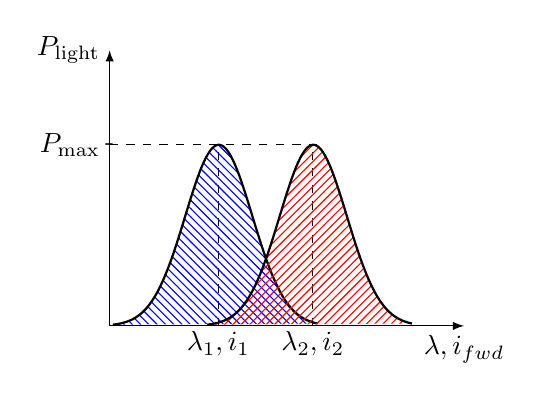
\begin{tikzpicture}

% horizontal axis
\definecolor{rrred}{rgb}{0.933, 0.227, 0.286}

\draw[->] (0,0) -- (4.5,0) node[anchor=north] {$\lambda,i_{fwd}$};
% labels
\draw	%(0,0) node[anchor=north] {0}
		(13.8mm,0.05) node[anchor=north] {$\lambda_1,i_1$}
		(25.8mm,0.05) node[anchor=north] {$\lambda_2,i_2$};
% ranges
%\draw	(1,3.5) node{{\scriptsize Constant flux}};
%		(4,3.5) node{{\scriptsize Field weakening}};
%\fill [draw=none, pattern=north west lines, pattern color=blue] (0,0) -- (2.40,0) -- (2.55,.45) -- cycle;
%\fill [draw=none, pattern=north east lines, pattern color=red] (2.42,0) -- (3.50,0) -- (3.50,3) -- cycle;
% vertical axis
\draw[->] (0,0) -- (0,3.5) node[anchor=east] {$P_\text{light}$};
% labels
\draw	%(0,0.6) node[anchor=east] {$P_{th}$}
		%(0,0.3) node[anchor=south] {-}
		(0,2.3) node[anchor=east] {$P_\text{max}$}
		(0,2.1) node[anchor=south] {-};

		
% nominal speed
%\draw[->,dotted] (2.60,0.61) --(2.41,0);
\draw[dashed] (13.8mm,0) -- (13.8mm,2.3);
\draw[dashed] (0,2.3) -- (26.5mm,2.3);
\draw[dashed] (25.8mm,0) -- (25.8mm,2.3);
%\draw[dashed] (0,0.5) -- (2.5,0.5);
%\draw[dashed] (0,3.0) -- (3.5,3.0);
% Us
%\draw[thick] (0,0) -- (2.49,0.46) -- (2.49,0.46) -- (2.61,0.61) -- (3.5,3) -- (3.71,3.5);
 \draw[thick,samples=100, domain=-11mm:15mm, pattern=north west lines, pattern color=blue] plot({\x+11.4mm},{-0.0+((2.3 * exp(-(\x/7 -1)^2/6)))}) ; 

 \draw[thick,samples=100, domain=-11mm:15mm, pattern=north east lines, pattern color=red] plot({\x+23.4mm},{-0.0+((2.3 * exp(-(\x/7 -1)^2/6)))}) ;
%\draw (1,1.5) node {$U_s$}; %label
%Y tick marks
%\foreach \x in {0,...,6}
%     		\draw (\x,1pt) -- (\x,-3pt)
%			node[anchor=north] {\x};
%    	\foreach \y in {0,...,4}
%     		\draw (1pt,\y) -- (-3pt,\y) 
%     			node[anchor=east] {\y}; 
% Psis
%\draw[thick,dashed] (0,3) -- (2,3) parabola[bend at end] (6,1);
%\draw (2.5,3) node {$\varPsi_s$}; %label

\end{tikzpicture}

\end{document}